%%%%%%%%%%%%%%%%%
% W tagging
%%%%%%%%%%%%%%%%%

One of the main highlights of the razor boost analysis is the tagging of boosted $\W$ bosons in
order to access a signal dominated phase space. 
$\W$ bosons either decay to two quarks, or to a lepton and a neutrino. The razor boost analysis is
an all-hadronic analysis, which means we do not explicitely consider the leptonic decays. 
$\W$ bosons with low to moderate transverse momentum will thus result in two jets, correponding to
the two clusters of particles resulting from the hadronization of the two quarks. 
As the $\pt$ of the $\W$ boson increases, the separation between the two resulting jets decreases.
For high enough momentum, the two jets can no longer be fully resolved with the usual jet
definitions, and will be reconstructed as a single jet. This turnover in efficiency between the
resolved and merged case is illustrated in Fig.~\ref{fig:boost_wtag_ca8eff}.
Depending on the requirements on the jet multiplicity, losing a jet can result in a loss of signal
efficiency. We can, however, also use this effect to our advantage, namely to increase the
signal-to-background ratio by requiring the presence of one of these \textit{merged} jets. 
This, in turn, allows us to relax the jet multiplicity requirements. 

\begin{figure}
  \centering
  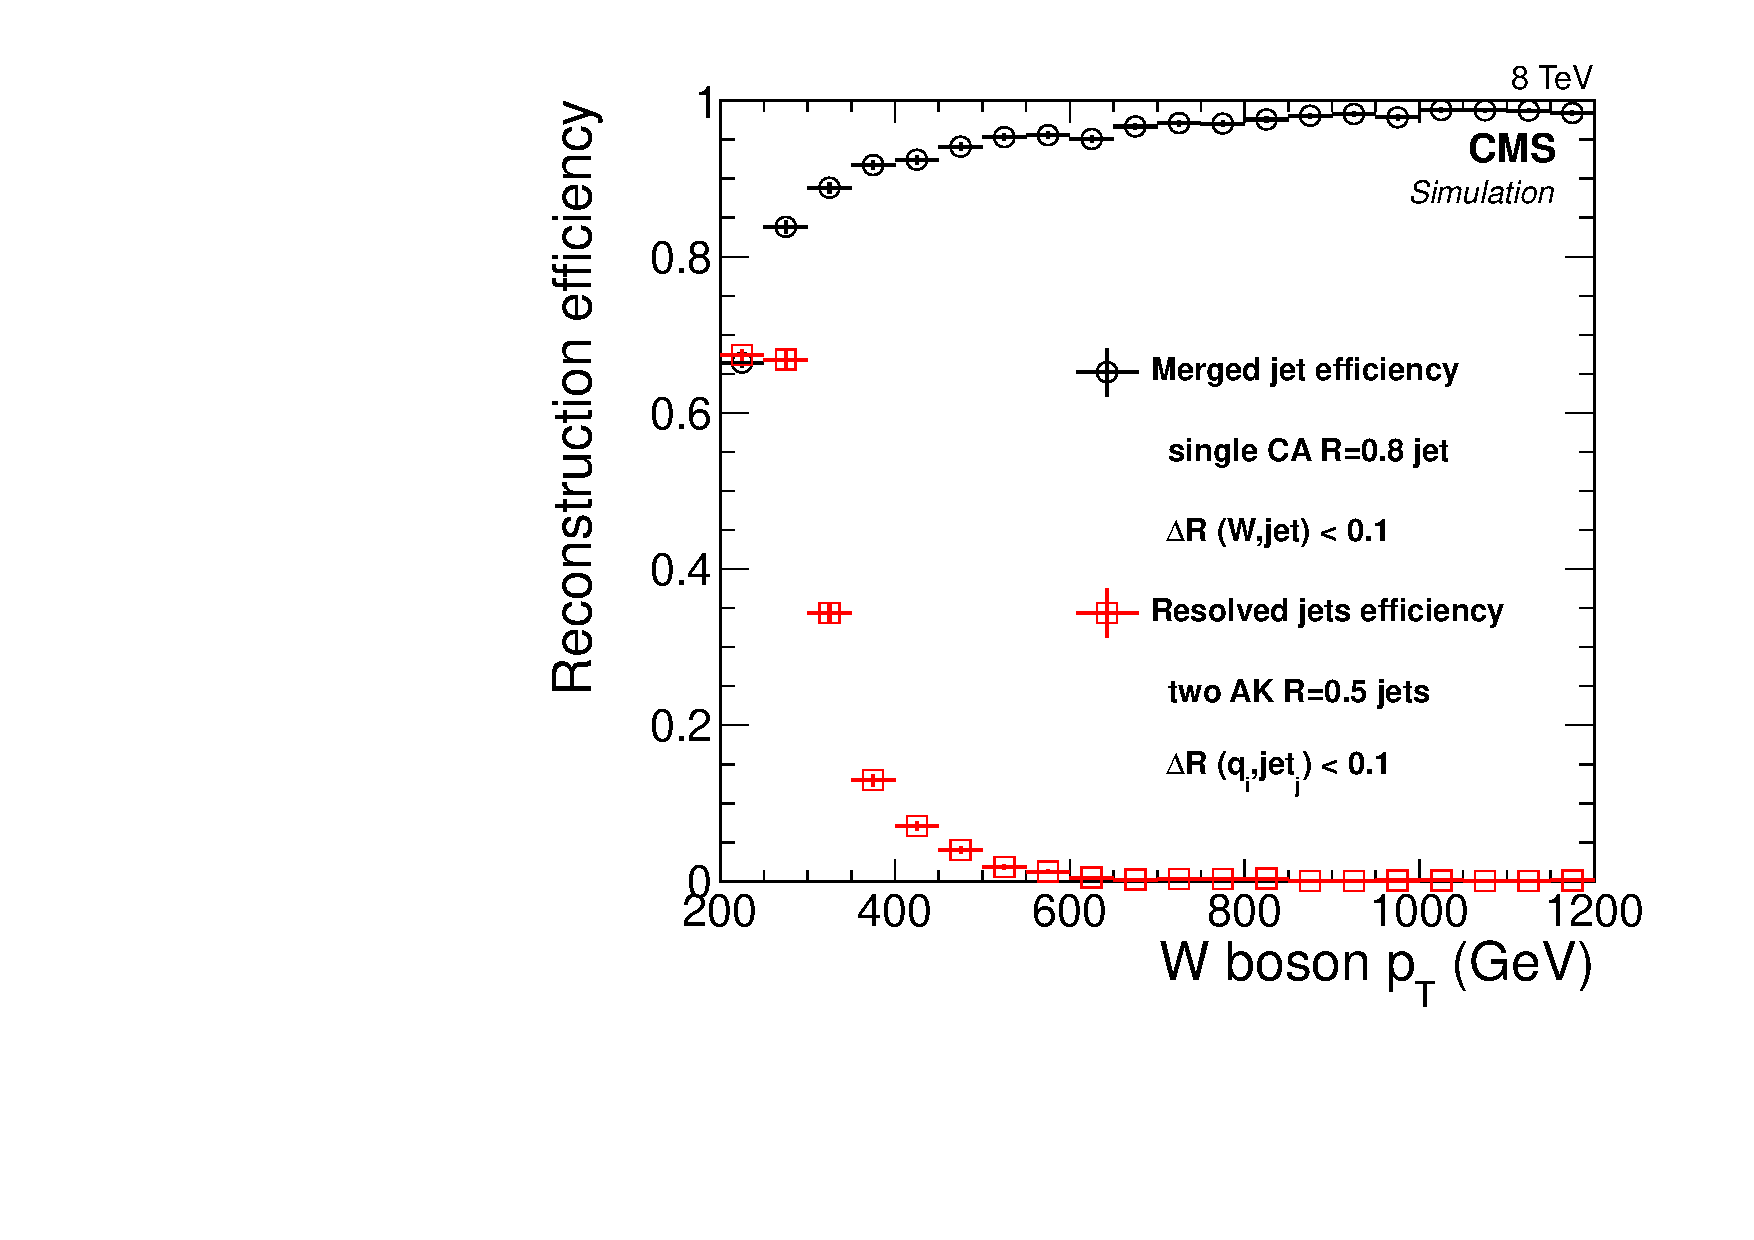
\includegraphics[width=0.7\textwidth]{figures/razor_wtag/ca8effVsPt}
  \caption{Efficiency to reconstruct a CA8 jet within $\Delta R<0.1$ of a generated $\W$ boson, and
the efficiency to reconstruct two AK5 jets within $\Delta R<0.1$ of the generated quarks from
longitudinally polarized $\W$ bosons, as a function of the $\pt$ of the $\W$
boson~\cite{Khachatryan:2014vla}. The loss in efficiency for the resolved case is clearly visible
for high $\pt$ $\W$ bosons. 
  \label{fig:boost_wtag_ca8eff}}
\end{figure}

The merged jet can be distinguished from other jets by its jet substructure, as illustrated in
Fig.~\ref{fig:boost_wtag_cartoon}. Jets originating from a $\W$ boson should have a two-prong
structure, whereas a quark/gluon-initiated jet is not expected to have this structure. 
In recent years, jet substructure techniques have seen very active developments, and many different
options are on the market~\cite{}. For the razor boost analysis we will use the CMS recommendation
in terms of which techniques to use~\cite{CMS-PAS-JME-13-006,Khachatryan:2014vla}. We will employ
\textit{jet pruning} and a set of variables called \textit{N-subjettiness}. On top of these jet
substructure techniques we will also use the jet mass variable to distinguish $\W$-initiated jets
from quark/gluon-initiated jets. 
The following subsections will go through the different parts of the
$\W$ tagging definition, providing a more detailed explanation for each. 
% TODO find jet substructure references

\begin{figure}
  \centering
  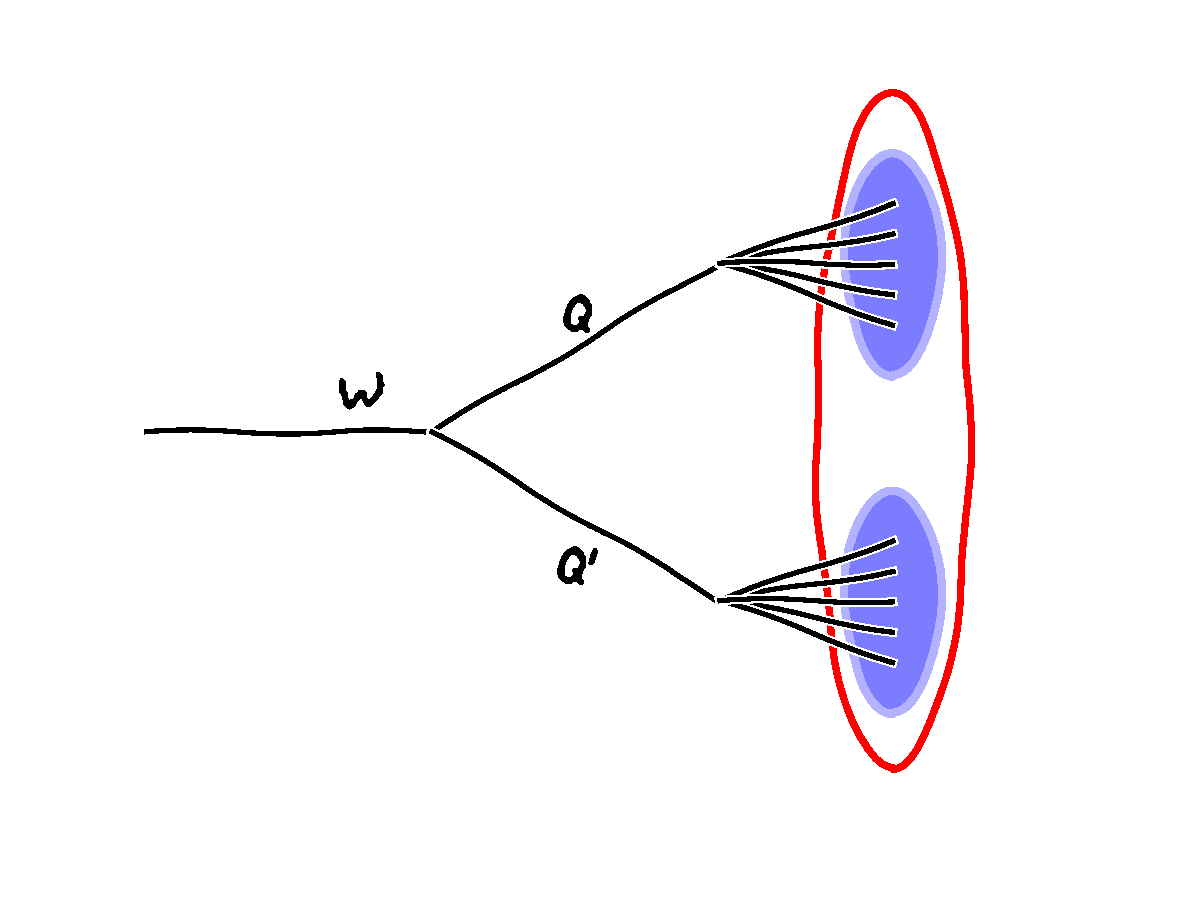
\includegraphics[width=0.48\textwidth]{figures/razor_wtag/W_subjets}
  ~
  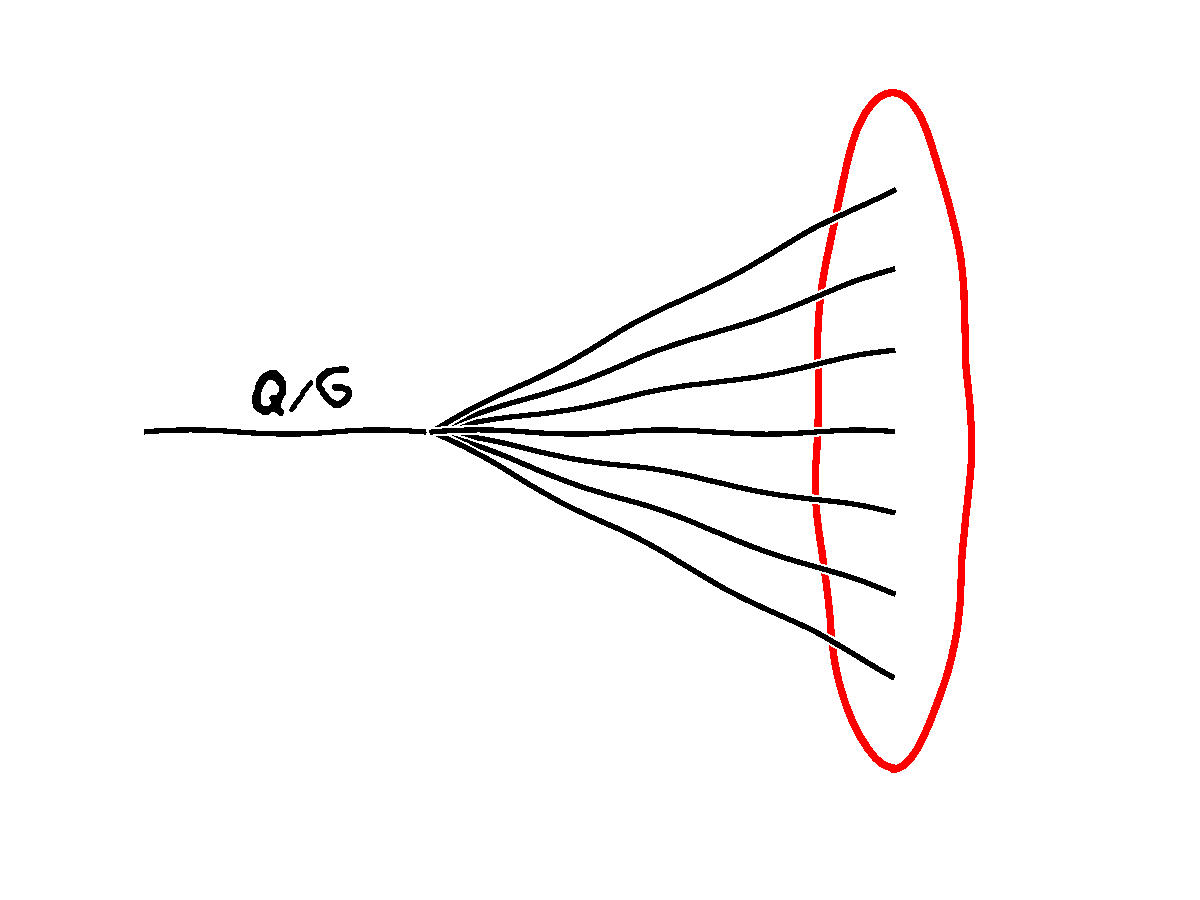
\includegraphics[width=0.48\textwidth]{figures/razor_wtag/qg_jets}
  \caption{The jet substructure of a $\W$-initiated jet differs from a quark/gluon-initiated jet.
  \label{fig:boost_wtag_cartoon}}
\end{figure}

%%%%%%%%%%%%%%%%%%%%%%%%%%%%%%%%%%%%%%%%%%%%%%%%%%%%%%%%%%%%%%%%%%%%%%%%%%%%%%%%%%%%%%%%%%%%%%%%%%%%

\subsection{Jet algorithm}

In order to identify boosted $\W$ bosons,  we will use a different jet clustering algorithm
than what is used for the standard jet definition (see Section~\ref{sec:object_jets}). 
Jets will be clustered with \textsc{FastJet 3.0.1.}~\cite{Cacciari:2011ma}, from the PF candidates,
using the Cambridge-Aachen algorithm~\cite{Dokshitzer:1997in} with a size parameter of 0.8.
Henceforth, we will call these jets \textit{CA8} jets. 

%\begin{quote}
\begin{cajet} \theoremstyle{definition}
The Cambridge-Aachen (CA) jet algorithm is a sequental recombination algorithm that uses the
distance measure $d_{ij}$ between two constituents $i$ and $j$,
\begin{equation}
d_{ij} = \frac{\Delta R_{ij}^2}{R^2}, \label{eq:CA_distance}
\end{equation}
with $R$ the size parameter of the resulting jets, and $\Delta R_{ij}^2 = (y_i - y_j)^2 + (\phi_i -
\phi_j)^2$ where $y, \phi$ are the rapidity and azimuthal angle. The rapidity is given in terms of
energy and longitudinal momentum as
\begin{equation}
  y = \frac{1}{2} \ln{\frac{ E + p_z }{ E - p_z }} .
\end{equation}
The distance between constituent $i$ and the beam is given by $d_{iB} = 1$.
As is clear from the above, these distance measures only use angular information, unlike for the
$k_T$ and anti-$k_T$ algorithms, which use a $\pt$-weighted distance. 

The jet algorithm starts by computing the minimum distance $d_{ij}$, across all $i,j$. If $\min
d_{ij} < d_{iB}$, then we combine constituents $i$ and $j$ into a new constituent whose
four-momentum is the sum of the four-momenta of $i$ and $j$, and repeat the process. Otherwise, we
call $i$ a jet and remove it from the list of constituents to be clustered. Again, the process is
repeated with the remaining constituents, until none remain.
\end{cajet}
%\end{quote}

Jet energy corrections for these CA8 jets are derived from the standard anti-$k_\textrm{T}$ jets
with size parameter $R=0.7$. Simulations show that the corrections are valid for CA8 jets and
have an additional uncertainty no greater than 2\%.  
% TODO find reference for this (some CMS study..)

%We require the CA8 jet mass to lie within the $\W$ boson mass range $70 < m_{jet} < 100$~\GeV
%and call such jets ``mass-tagged" ($Y$).  

%Subjets are obtained by
% undoing or reversing the last step of the clustering algorithm.  



%%%%%%%%%%%%%%%%%%%%%%%%%%%%%%%%%%%%%%%%%%%%%%%%%%%%%%%%%%%%%%%%%%%%%%%%%%%%%%%%%%%%%%%%%%%%%%%%%%%%

\subsection{Jet pruning}

Jet pruning~\cite{Ellis:2009su,Ellis:2009me} is a particular kind of jet grooming. Jet grooming
techniques are designed to reduce the impact of contributions from the underlying event (UE), pileup
(PU), and low-\pt gluon radiation. These kinds of contributions to jets are typically soft and
diffuse, and increase the jet energy proportional to the jet area. Grooming techniques reduce the
jet area without affecting the core components. This means that the resulting jets are less
sensitive to these soft contributions, but still reflect the kinematics of the original, hard
process.


During jet pruning the constituents of the jet are reclustered through the CA algorithm, using the
same distance parameter as used for the original jets (here $R=0.8$), but with additional conditions
beyond those of the standard algorithm.
In particular, the softer and larger-angle of the two particles $i$ and $j$ to be merged is removed
when the following conditions are satisfied:
\begin{align}
  z_{ij} &= \frac{\min( \pt^i , \pt^j )}{\pt^i + \pt^j} < z_{\textrm{cut}}, \\
  \Delta R_{ij} &> D_{\textrm{cut}} \equiv \alpha \frac{m_J}{\pt} ,
\end{align}
where $m_J$ and $\pt$ are the mass and transverse momentum of the originally-clustered jet, and
$z_\textrm{cut}$ and $\alpha$ are parameters of the algorithm, chosen to be 0.1 and 0.5,
respectively~\cite{Chatrchyan:2013vbb}. 

The resulting pruned jet is used as further input to our $\W$ tagger. For the $\W$ decay products
to be collimated, we need a large transverse momentum. We will therefore require that the pruned
jets have $\pt > 200\GeV$. 
Because of the reduction of the effect of UE and PU, the jet mass variable as computed from the
constituents of the jet after jet pruning has a much better behavior than if it was computed from
the unpruned jets, see Fig.~\ref{fig:wtag_jet_pruning}. 
We will make the requirement that the pruned jet mass is consistent with the $\W$ boson mass.
\begin{equation}
  70 < m_{\textrm{pruned jet}} < 100 \GeV
\end{equation}
This provides good boosted $\W$ jet to quark/gluon jet discrimination. 

\begin{figure}
  \centering
  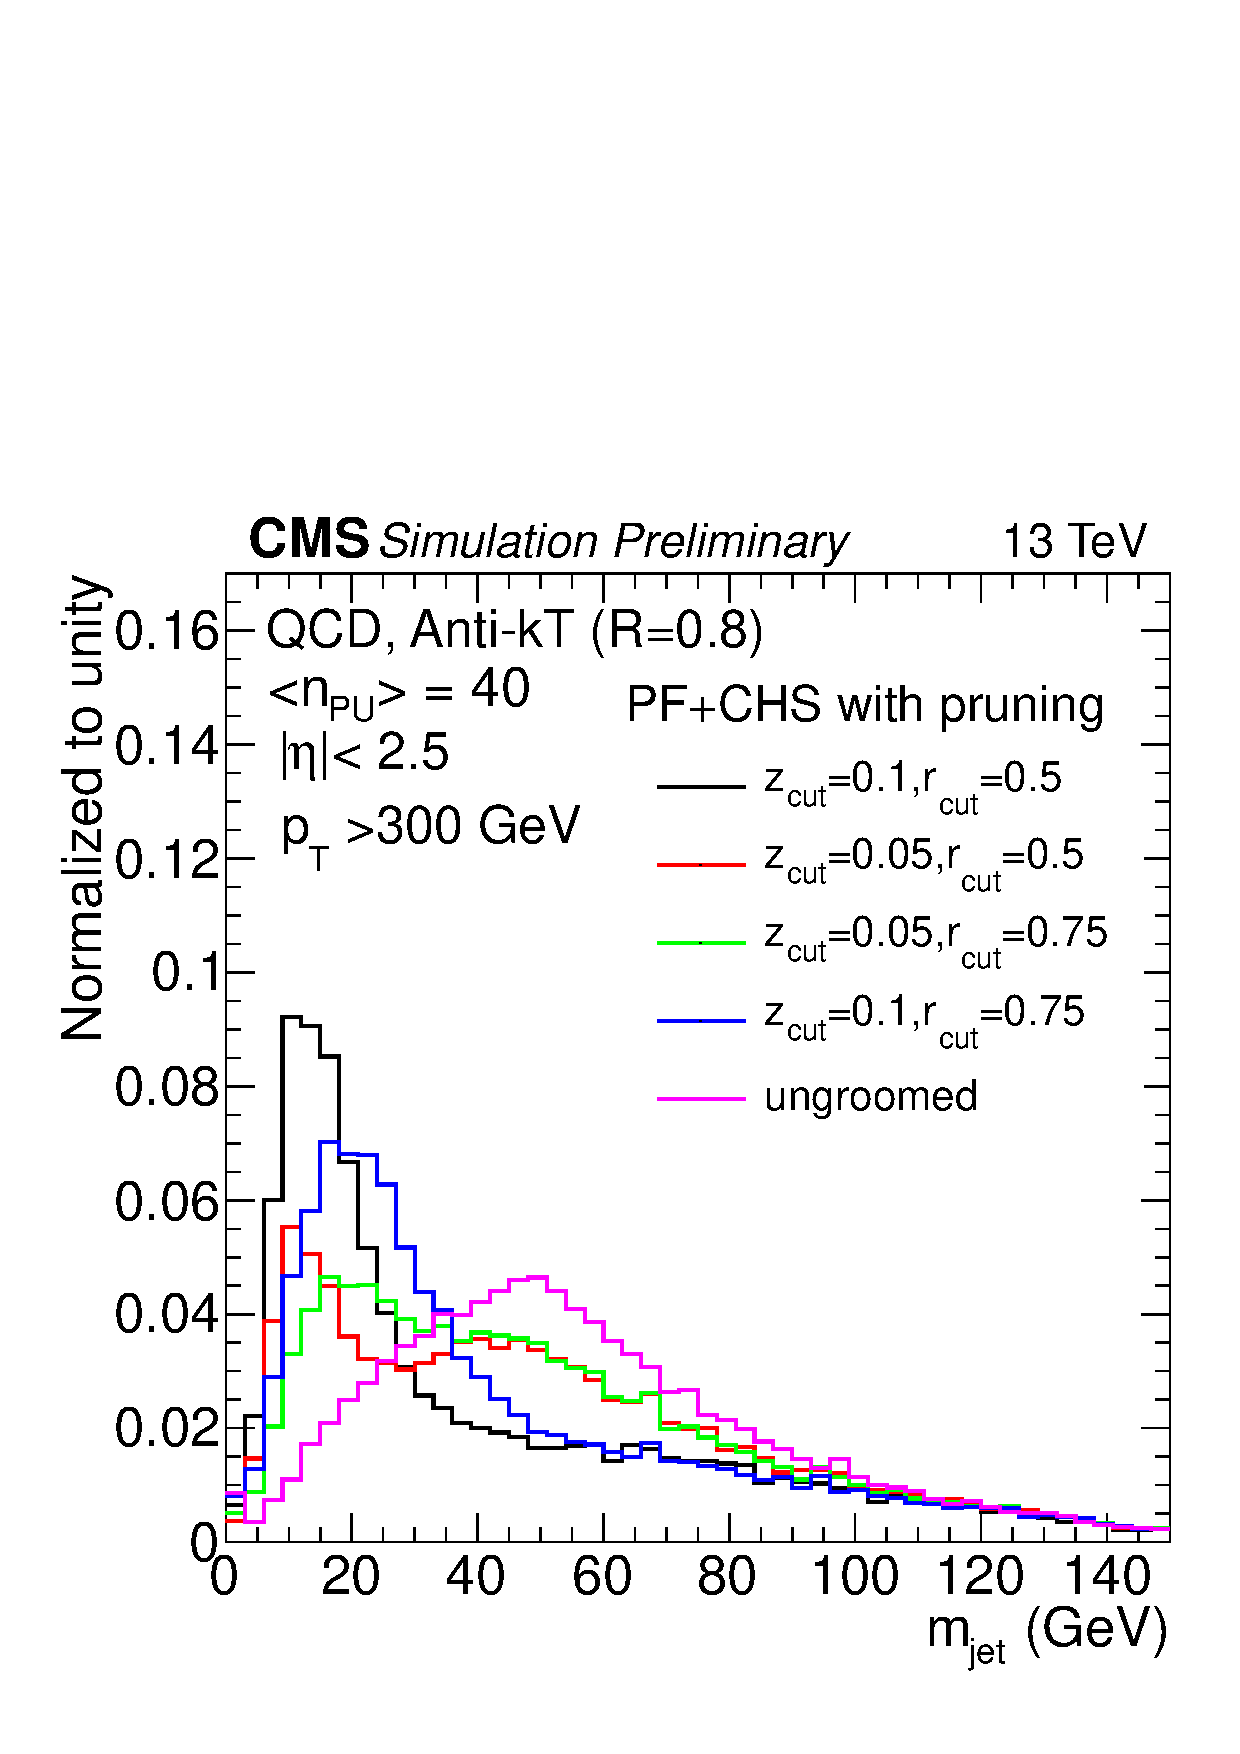
\includegraphics[width=0.6\textwidth]{figures/razor_wtag/1DPFCHS_PR_QCD}
  \caption{Jet mass distribution of QCD jets with $\pt(\textrm{gen}) > 300 \GeV$ for various
groomers (PF+CHS jets). The ungroomed mass distribution is also shown for
comparison~\cite{CMS-PAS-JME-14-001}. 
  \label{fig:wtag_jet_pruning}}
\end{figure}


\subsection{N-subjettiness}

Given $N$ candidate subjets, obtained with \textsc{FastJet} via exclusive $k_T$ clustering with a
one-pass optimization, in a given CA8 jet, the N-subjettiness variables~\cite{Thaler:2010tr} are
computed as follows, 
\begin{equation}
\tau_N = \frac{1}{R_0 \sum_{k} p_{T, k}} \sum_k p_{T, k} \min (\Delta R_{1,k}, \Delta R_{2,k}, ...
\Delta R_{N,k}),
\end{equation}
where $R_0$ is the original jet size parameter (0.8 in our case) and $k$ runs over all constituent
particles. 

The variables $\tau_N$ quantify the consistency of the jet having $N$ subjets. They can be viewed
as a distance measure, and are small (close to 0) if the original jet is consistent with having $N$
subjets. As we are interested in discriminating boosted $\W$ bosons from quark/gluon jets, we will
use the variables $\tau_2$ and $\tau_1$. 
It has been shown that the ratio of the $\tau_N$ variables are better discriminitors than the
separate variables. We will require that the ratio $\tau_2 / \tau_1$ is small.


\subsection{\texorpdfstring{$\W$}{W} tagging definitions}

Therefore, in order to discriminate boosted $\W$ bosons, which have two subjets, from q/g jets,
characterized by a single subjet, we require $\tau_2 / \tau_1 < 0.5$.  The complement of this
selection defines anti-tagged $\W$ jets ($aW$), which are used in the definition of control regions
that are used in the background modelling.

\cite{EXO-12-024,CMS-PAS-JME-13-006}

The CMS Collaboration has investigated several jet substructure techniques and has developed a
recommended boosted boson tagger using the N-subjettiness variables~\cite{Thaler:2010tr}. This
study
is documented in~\cite{CMS-PAS-JME-13-006}.  
Several EXO analyses have already used this W tagger~\cite{EXO-12-024,EXO-13-009}.

A summary of the boosted $\W$ tagger definition is shown in table~\ref{tab:Wtag_definition}. 

% TODO: think about how much detail I want here (collection names?)
\begin{table}[htdp]
\caption{Boosted $\W$ tagging definition}
\centering
\begin{tabular}{|ll|}
\hline
\multicolumn{2}{|l|}{CMSSW collection label: selectedPatJetsCA8CHSpruned} \\
\multicolumn{2}{|l|}{CMSSW type: pat::Jet} \\
\hline
Variable/Method & Value \\
\hline
pt() & $> 200$ \\
fabs(eta()) & $< 2.4$ \\
mass() & $70-100$ \\
\hline
\multicolumn{2}{|l|}{CMSSW collection label: selectedPatJetsCA8CHSwithQjets} \\
\hline
tau2()/tau1() & $< 0.5$ \\
\hline
\end{tabular}
\label{tab:Wtag_EXO}
\end{table}



%%%%%%%%%%%%%%%%%%%%%%%%%%%%%%%%%%%%%%%%%%%%%%%%%%%%%%%%%%%%%%%%%%%%%%%%%%%


\subsubsection{\texorpdfstring{$\W$}{W} mass tagging and \texorpdfstring{$\W$}{W} anti-tagging
\label{sec:W_mass_anti_tagging}}

The $W$ tagger defined above will be used to select events in the signal region and in the TTJets
control region (see section~\ref{sec:Sregion} and \ref{sec:Tregion}). In both of those regions, we
expect to have real hadronically decaying $\W$ bosons, mainly coming from the $t\bar{t}+$jets
background. 

Another background in the signal region, is QCD multijet production, for which we have defined a
dedicated control region (section~\ref{sec:Qregion}). Multijet events do not have real $\W$ bosons;
any CA8 jet that passes the W tagger, is thus by definition a misidentified or \textit{fake} $\W$. 
For the QCD control region we define ``anti-tagged $W$'s'' ($aW$), in which we invert the
n-subjettiness cut but leave the other cuts the same. 
As we do not expect QCD events to have the two-prong jet-substructure of actual boosted $W$'s, this
will enhance the statistical power of the control region. 

Our final background in the signal region for which we have a dedicated control region, is
$\W(\rightarrow l\nu)$+jets. 
As the $\W$ boson decays leptonically, any events passing the signal selection must contain a CA8
jet that is misidentified as a boosted $\W$. 
We do not expect hadronically decaying $\W$ bosons to be a large background, as those events would
usually not come with $\cPqb$-jets, and would have very small missing energy. Even though we do not
explicitely require a minimal \ETm, our $R^2$ cut is highly correlated with \ETm, and induces
a minimal cut of around 100\GeV, as can be seen in figure~\ref{fig:DataMC_SignalRegion_mdphig0p5}.  
We have verified this assumption by checking the contribution of $\W(\rightarrow
q\bar{q}')+b\bar{b}$ using simulation, and found that no events pass our signal selection. 
For the $W$+jets control region, which is defined by requiring the presence of a lepton, we only
keep the mass window requirement to select CA8 jets that fake a boosted $\W$ boson. We will denote
these mass-tagged $\W$'s as $Y$. We do not use any cut on the n-subjettiness variables to increase
the number of events available in the control region. 

As a summary, we show both the ``anti-tagged'' and ``mass-tagged'' definitions in
table~\ref{tab:Wtag_mass_anti}.

\begin{table}[htdp]
\caption{$W$ mass-tagging and anti-tagging definition}
\begin{center}
\begin{tabular}{|l|c|c|}
\hline
\multicolumn{3}{|l|}{CMSSW collection label: selectedPatJetsCA8CHSpruned} \\
\multicolumn{3}{|l|}{CMSSW type: pat::Jet} \\
\hline
Variable/Method & Value mass-tagger & Value anti-tagger \\
\hline
pt() & \multicolumn{2}{c|}{$> 200$} \\
fabs(eta()) & \multicolumn{2}{c|}{$< 2.4$} \\
mass() & \multicolumn{2}{c|}{$70-100$} \\
\hline
\multicolumn{3}{|l|}{CMSSW collection label: selectedPatJetsCA8CHSwithQjets} \\
\hline
tau2()/tau1() & - & $> 0.5$ \\
\hline
\end{tabular}
\end{center}
\label{tab:Wtag_mass_anti}
\end{table}

Data/MC scale factors for these definitions are also needed. They are not provided centrally, so we
derived them ourselves. For more details we refer to section~\ref{sec:wtag_scale_factor}. In that
section we also show how we derive a FullSim/FastSim scale factor and a scale factor for the W-tag
fake rate. 


\subsection{\texorpdfstring{$\W$}{W} tagging scale factors \label{sec:wtag_scale_factor}}


It has been observed by previous CMS analyses that the $\W$ tagging efficiency is not the same in
data and in simulation. To account for this, Data/MC scale factors have been derived, following the
method outlined in Ref.~\cite{CMS-PAS-JME-13-006}.
The $\W$ tagging efficiency scale factor which we will use in our analysis, was published in the
EXO-12-024 paper~\cite{EXO-12-024}, and is given by: 
\begin{equation}
SF_{\textrm{Wtag}} = 0.86 \pm 0.07 .
\end{equation}
For our signal samples, which are produced with FastSim, we have derived an additional $\W$ tag
efficiency FullSim/FastSim scale factor. The product of
$SF_{\textrm{Wtag}}$ and the FullSim/Fastsim scale factor will be applied to the signal simulation. 

% TODO add the fullsim/fastsim stuff

% TODO add the other scale factor
% explain the wiggle
